\documentclass[12pt,letterpaper]{article}

%==================================================================================
% Template for the 13th International Association of Fire Safety Science (2019).  
%==================================================================================

% This template is based on the layout requirements of the Fire Safety Journal.  When submitting, please do include the *.tex and output (typeset) *.pdf files, figure files (photographs, diagrams, etc.), and any other ancillary files required to typeset your article.  The journal must be able to typeset your article with what you've provided.

% As with any programming language, there are multiple ways of executing any given task (e.g., figures, tables, maths, etc.).  The syntax in this template should be considered suggestions and not directives.  Please feel free to use your own favorite syntax, especially if it's more elegant than what is found below!  That said, the spacing and font parameters have been selected to conform to the appearance dictated by the journal (i.e. like MS Word).  Make sure your final typeset document has the correct formatting or it will be rejected.

% Required Packages ===============================================================
\usepackage{amsmath} % The usual maths package
\usepackage{amsfonts}  % The usual maths package
\usepackage{amssymb}  % The usual maths package
\usepackage[final]{graphicx} %Required for figures.
\usepackage{footnote}
\usepackage{footmisc}
\usepackage{caption} % Needed to modify default figure captions
\usepackage{latexsym}
\usepackage{lineno} % Enables line numbers
\usepackage{parskip} % Makes a space between paragraphs like MS word
\usepackage{fullpage} % Overrides article margins
\usepackage{titlesec} % Enables modification of section labels
\usepackage[numbers,sort&compress]{natbib}
%\usepackage[numbib]{tocbibind} %Make References a numbered section
\usepackage{siunitx} % Formats the units and values
\usepackage{times}
\usepackage{chemformula}


%\usepackage{subcaption} % Enables multiple images in one figure environment
%\usepackage{xcolor} % For various font colors in figures
%===================================================================================

% The next two lines modify the font and font size of the section and subsection labels
\titleformat{\section}{\normalfont\bfseries}{\thesection}{0.2em.}{}
\titleformat{\subsection}{\normalfont\bfseries}{\thesubsection}{0.2em}{}

% This will change the figure captions from the default "Figure 1:" to "Fig. 1."
\captionsetup[figure]{labelformat={default},labelsep=period,name={Fig.}}

\linenumbers % Include line numbers throughout document

\newcommand\numberthis{\addtocounter{equation}{1}\tag{\theequation}}

\begin{document} %====================================================================
\begin{flushleft} % Suppress the default full justification of text

% Title of your article
\textbf{A study on local conditions conducive to deflagration in a scaled compartment}
\vspace{3mm}\\
%
% Author(s)
Marcos Vanella$^\text{a*}$, Chandan Paul$^\text{a,b}$, Thomas Cleary$^\text{a}$, Ryan Falkenstein-Smith$^\text{a}$
\vspace{3mm}\\	

% Affiliation "b"
$^\text{a}$National Institute of Standards and Technology, 100 Bureau Drive, Gaithersburg, USA  \\
$^\text{b}$The George Washington University, 800 22nd Street, NW, Washington DC, USA  \\
\vspace{3mm}

$^*$Corresponding author : marcos.vanella@nist.gov

% Highlights/keywords ===================================================
%\textbf{Highlights:}	
%\begin{itemize}
%	\itemsep-4pt % Override default vertical spacing among list items
%	\item A series of backdraft experiments were conducted in a reduced-scale enclosure
%	\item Different methane and propane fire configurations were implemented to vary the gas mixture distribution and internal density
%	\item The gas mixture density within the enclosure was observed to impact the mixing dynamics of the gravity current as it entered the compartment
%	\item Ignition was achieved for rich gas mixtures surrounding a charged spark ignitor
%	\item \textcolor{black}{A relationship between the total heat release of the resulting backdraft and the initial mass fraction of fuel residing within the enclosure was observed} for experiments utilizing propane
%\end{itemize}
%\vspace{3mm}

% Abstract ==============================================================	
\textbf{Abstract:}

\vspace{3mm}


\textbf{Keywords:}
Enclosure Fire; Gaseous Fuels; Backdraft; Experiments; Numerical Simulation

\section{Introduction} \addvspace{10pt}
\label{sec:introduction}
Backdraft occurs when air, driven by a gravity current, is introduced to a fuel-rich and oxygen-depleted isolated heated enclosure that then mixes and ignites, resulting in a deflagration projected outside of the enclosure. Several works have studied physical mechanisms such as compartment size and vent configurations~\cite{weng2002study,weng2005experimental,weng2005prediction}, internal thermochemical properties~\cite{Chen2012,gong2006theoretical}, and critical conditions for the development of the gravity current driven airflow~\cite{fleischmann1993backdraft,fleischmann1994quantitative,fleischmann1993exploratory}.

Most research focuses on investigating backdraft phenomenon on a global level, generalizing the internal conditions of the compartment. Gottuk et al. investigated a critical fuel mass required to develop a backdraft~\cite{gottuk1999development,farley1997development}. Tseng et al.~\cite{tseng2024effect} developed a critical temperature for their compartment configuration for backdraft to occur. Although generalizations of internal conditions conducive to backdraft provide insight into relationships between parameters and the resulting phenomenon, they are not practical in the sense of providing a realistic approach to determining the likelihood of the threat. 

For example, Ref.~\cite{chen2011theoretical} established a theoretical approach to determining backdraft using gas concentration measurements, under the assumption of well-mixed internal conditions. Falkenstein-Smith et al., however, demonstrated that fuel distribution varies with sampling location. As opposed to determining critical conditions resulting in backdraft via generalization of the internal conditions, a stronger approach to understanding the phenomenon is accounting for more realistic conditions and understanding how they influence the phenomenon. 

In this work, experimental conditions are taken from Refs.~\cite{falkenstein2023gas,Falkenstein2022} and incorporated into a computational fire model to understand how temperature, fuel, and oxygen distribution within an enclosure influences backdraft generation. 


Backdraft - what it is, lit review. Local conditions conducive to flame propagation within the compartment. Mixing, critical fuel mass.

- Simulations, lit review, 2-3 equation kinetics for combustion, arrhenius vs fast chemistry.

- Purpose of this work - study flame propagation potential comparing to experiments done at NIST. We are talking about deflagration initiation with spherical flame with diameter up to several centimeters. In this scenario fully mixed fuel and oxygen can be assumed. Other than that, the flame will move into regions where combustion can be mixing controlled (into the gravity current) and pressure generation affects the dynamics of the compartment ejecting fuel, oxygen and products through the door. What affects the flame viability? Do profiles of temperature, fuel, initial Oxygen with height have an effect? 

\section{Experimental Setup} \addvspace{10pt}
\label{sec:expsetup}
Experiments were conducted in 1.0~m x 1.0~m x 1.5~m reduced-scale enclosure. The enclosure’s front had a pneumatically operated door along a short wall with a 43.0~cm wide and 80.0~cm high opening. A 3.8~cm diameter vent was constructed in the lower right wall of the compartment, 38.0~cm from the front interior wall of the compartment, and 3.0~cm above the compartment floor. The vent's purpose was to prevent overpressure within the compartment by allowing a uniform leakage area when the door is closed. A detailed description of the compartment is available in Ref.~\cite{Brown2022}.
Figure~\ref{fig:Backdraft_experimental_setup} provides a schematic of the compartment with a gas burner, spark igniters, gas sampling probes, and thermocouples positions. A 17.8~cm square sand burner was centered approximately 1.25~m from the compartment opening and 0.5~m from either side wall. The bottom of the burner was connected to a mass flow controller (MFC) via a fuel line to control the fire size within the compartment. 

Backdraft ignition was initiated from a spark ignitor positioned at the height of either 25.4~cm (``low spark'') or 50.7~cm (``mid spark'') from the compartment floor, respectively. Every experiment incorporated a 10.8~cm long and a 55.9~cm long spark ignitor located on the left and right walls of the compartment, respectively, in either the low or mid spark position. 

The reduced-scale enclosure included two K-type thermocouple arrays positioned on opposing walls of the compartment. The first thermocouple array was spaced in a line, 19.9 cm apart, on the right wall facing the door using four 0.3175 cm (nominally 1/8”) diameter sheathed Type K thermocouples, 24.8 cm long. The second thermocouple array was positioned in a rectangular orientation on the left wall facing the door, using 0.3175 cm (nominally 1/8”) diameter sheathed Type K thermocouples, 49.5 cm long. 

Gas samples were continuously extracted, approximately at the center of the compartment, only using two gas sampling positions for each experiment. Extracted gas samples were portioned into a gas analyzer and a second-generation phi meter. The gas analyzer included one paramagnetic sensor for oxygen concentration measurements, and two non-dispersive infrared non-dispersive infrared (NDIR) sensors to measure carbon dioxide and carbon monoxide concentrations. The second-generation phi meter provided a local measurement of the global, $\phi_{\rm{G}}$, and local fuel, $\phi_{\rm{LF}}$, equivalence ratio, as defined in Ref.~\cite{falkenstein2023equivalence}. All measurements described here were recorded using a data acquisition system (DAQ) maintained at a sampling rate of 1.0 Hz. 

\subsection{Experimental Procedure} \addvspace{10pt}
\label{sec:procedure}
Backdraft experiments were initiated when a small flow of propane, controlled via the MFC,  was fed into the burner, burned, and then ignited using a propane wand (t=0). After ignition, the propane flow was adjusted to approximately 25.0~kW~$\pm$~1.0~kW. For the first 60~s after ignition, the fire burned while the compartment doorway remained open, allowing the flame to reach a quasi-steady state. After a minute from the ignition, the compartment opening was closed, while fuel continued to be fed into the burner until it was shut off once a predetermined fuel flow time was achieved (t=fuel flow time). For the 25.0~kW propane fire, fuel flow times of either 210~s, 240~s, 270~s, or 300~s were used. The doorway remained closed for an additional 30~s after the fuel flow time, after which the doorway opened, and a potential backdraft was observed (t=fuel flow time+30).

\subsection{Definition of Initial Conditions} \addvspace{10pt}
\label{sec:initcond}
Temperature and species concentration profiles were estimated from time-averaged measurements at various heights in the compartment. Time-averaged temperature readings and gas concentrations were established from the average of measurements taken 10~s prior to the compartment door opening (t=fuel flow time+20:fuel flow time+30). In this work, it is assumed that temperature and gas mixture composition vary only in height. This assumption is supported by the small variation in temperature and gas concentration readings between the front and rear of the compartment. 

Gas mixture composition was assumed to include only propane, oxygen, carbon dioxide, carbon monoxide, water vapor, and nitrogen. The second-generation phi meter's ability to measure $\phi_{\rm{LF}}$, combined with the gas analyzer's oxygen concentration measurement, provided an estimate for the propane mole fraction, assuming the stoichiometry of propane. The concentration of water vapor was approximated from a combination of the carbon dioxide and carbon monoxide measurements obtained in the gas analyzer, assuming the carbon-to-hydrogen atom ratio of propane. The remainder of the gas mixture was assumed to be inert.



\begin{figure}[H]
    \centering
    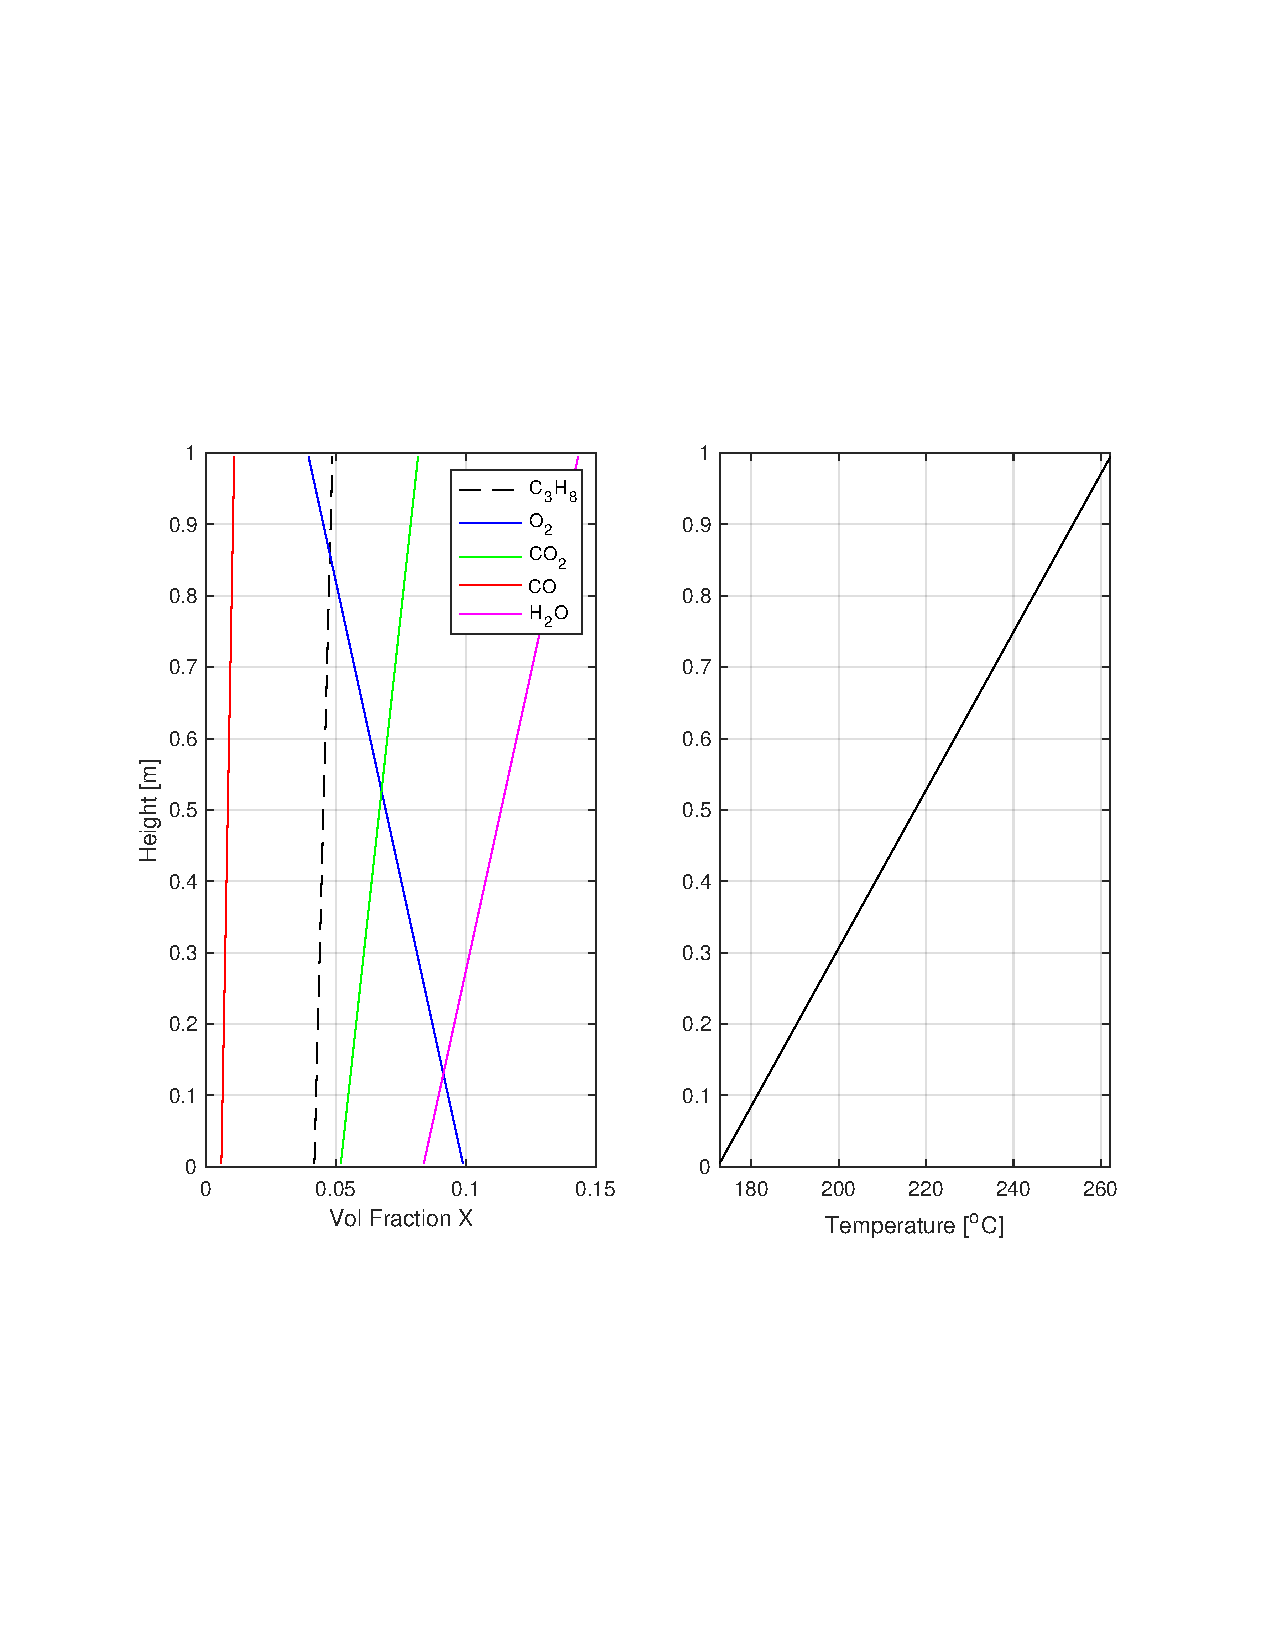
\includegraphics[trim = 22mm 70mm 27mm 72mm, clip,width=0.49\textwidth]{AOSFST_Paper/Figures/CompositionTemp_FFT_210s}
    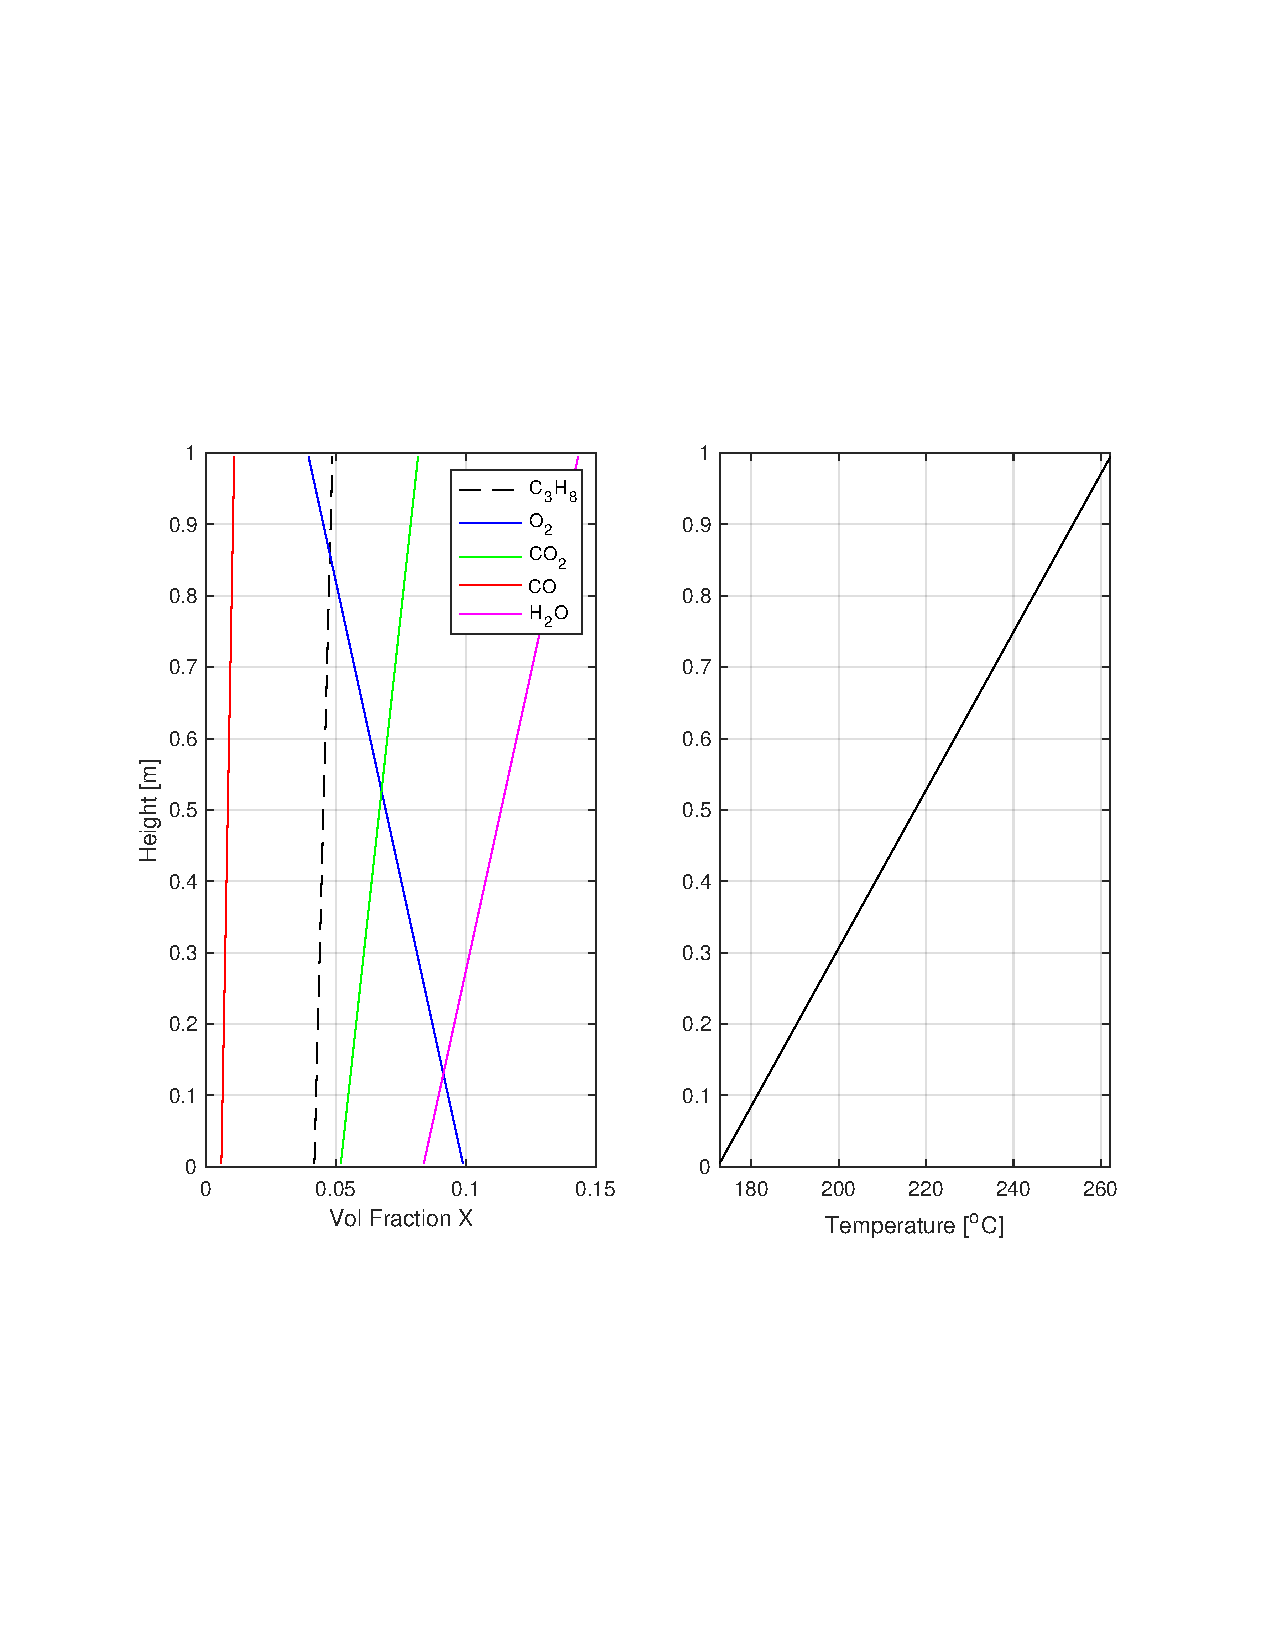
\includegraphics[trim = 22mm 70mm 27mm 72mm, clip,width=0.49\textwidth]{AOSFST_Paper/Figures/CompositionTemp_FFT_210s}
    \makebox[0.50\textwidth]{(a)}
    \makebox[0.48\textwidth]{(b)} \\
    %\caption{Initial composition and Temperature profiles: (a) FFT=210 s (b) FFT=240 s. }
    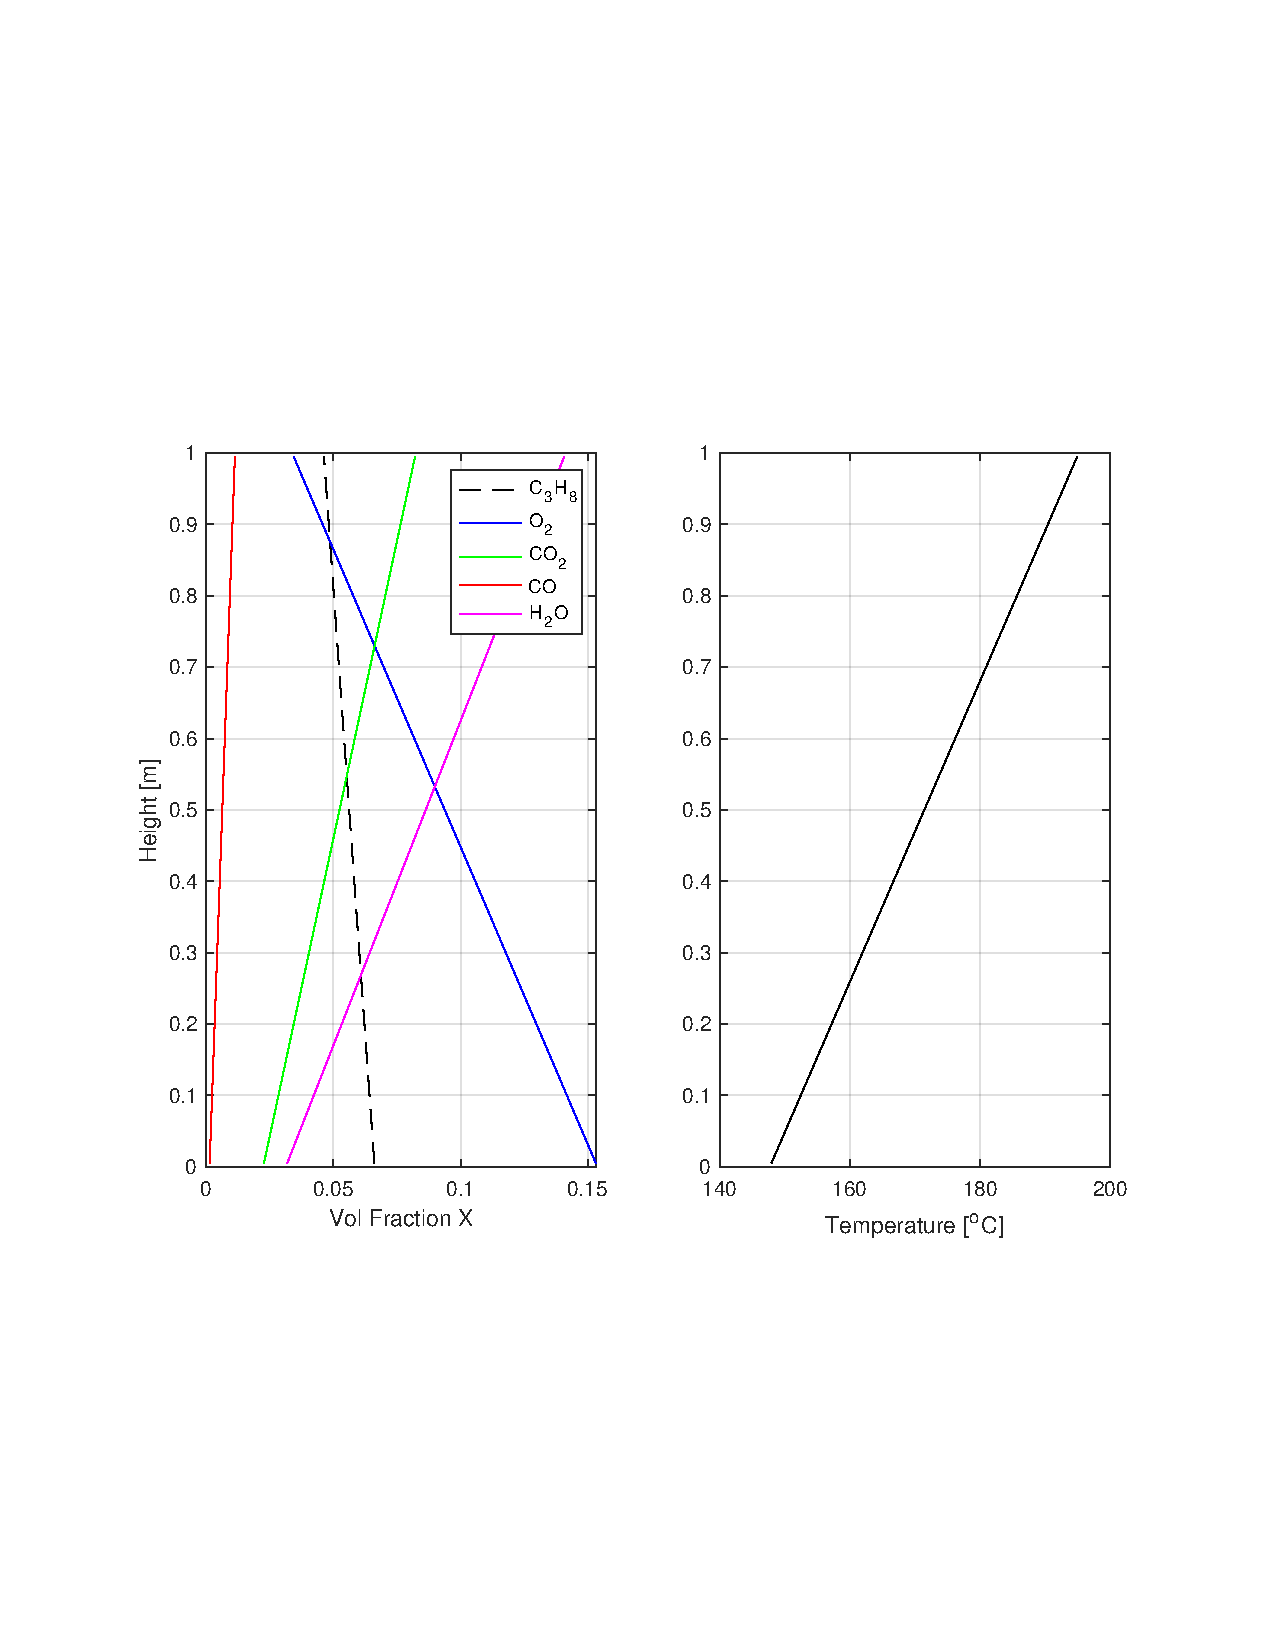
\includegraphics[trim = 22mm 70mm 27mm 72mm, clip,width=0.49\textwidth]{AOSFST_Paper/Figures/CompositionTemp_FFT_270s}
    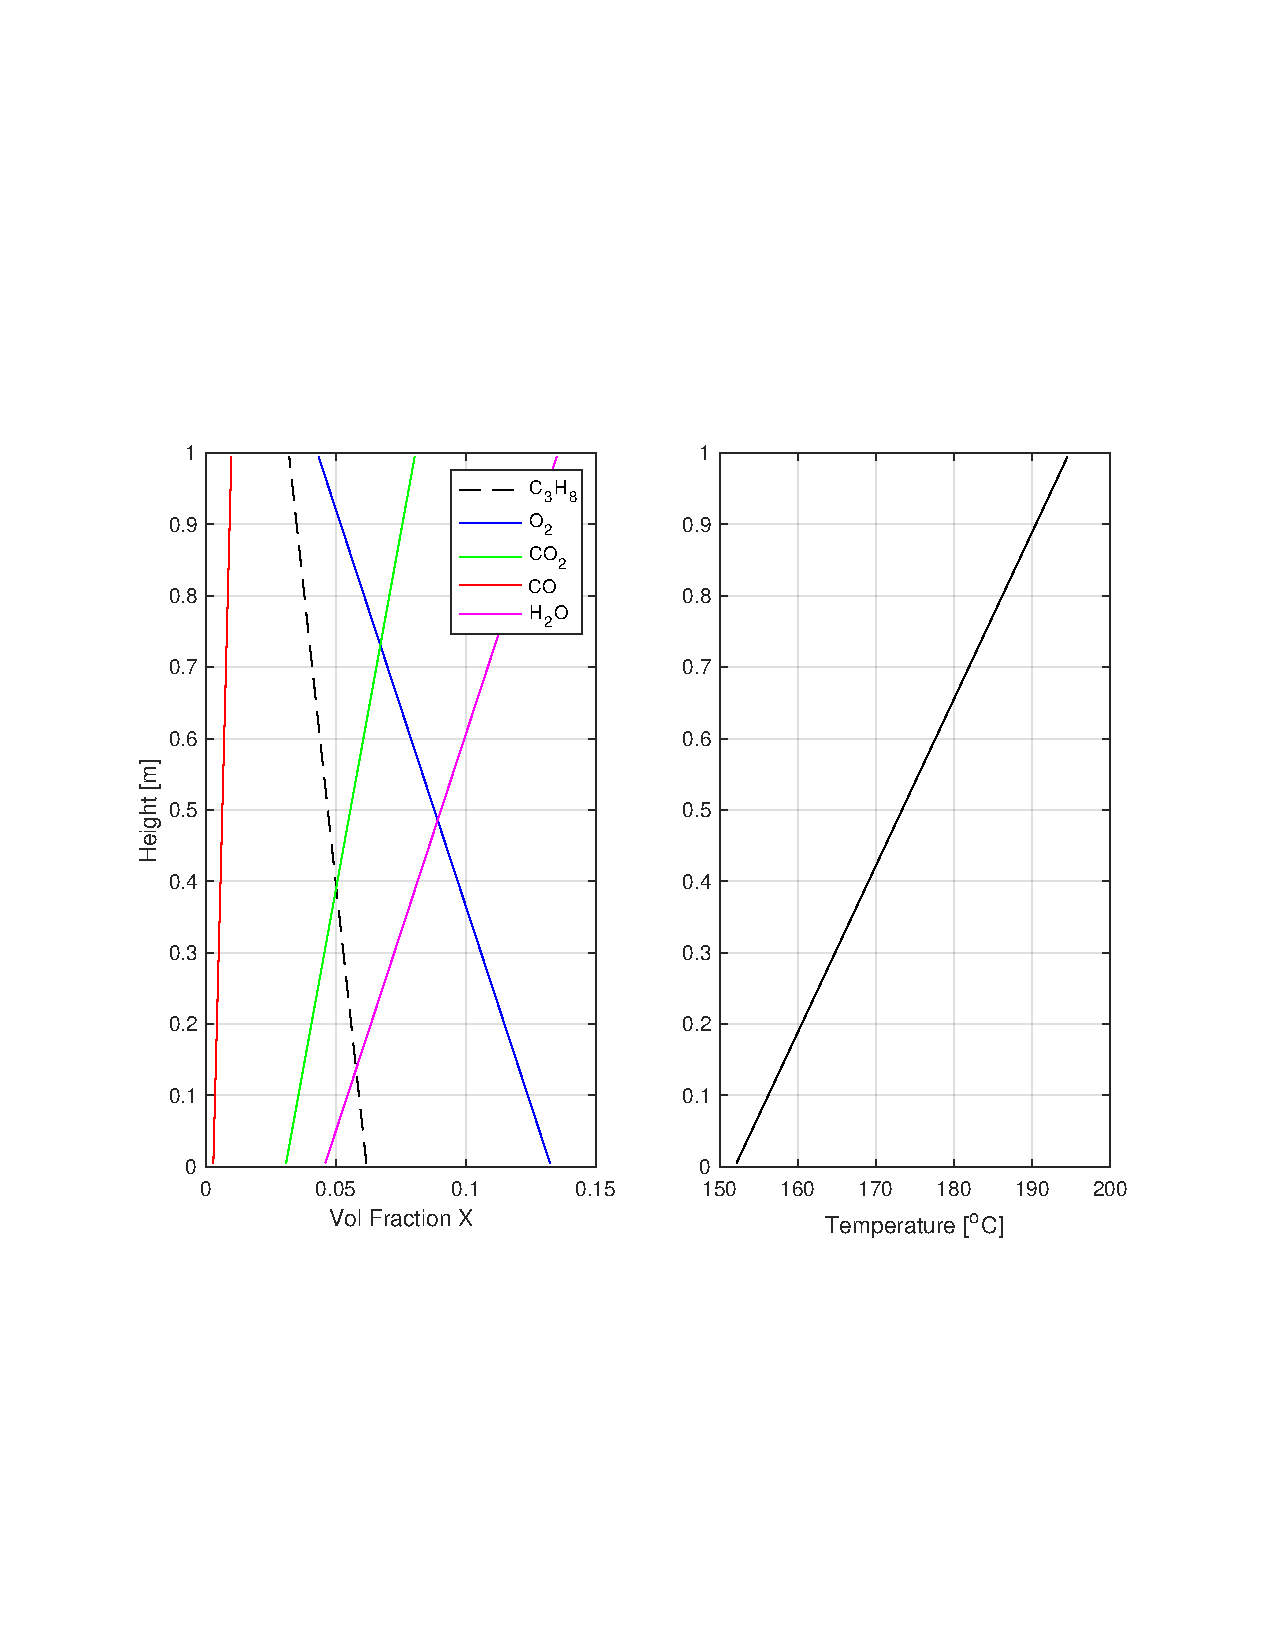
\includegraphics[trim = 22mm 70mm 27mm 72mm, clip,width=0.49\textwidth]{AOSFST_Paper/Figures/CompositionTemp_FFT_300s}
    \makebox[0.50\textwidth]{(c)}
    \makebox[0.48\textwidth]{(d)} \\
    \caption{Initial composition and Temperature profiles: (a) FFT=210 s (b) FFT=240 s (c) FFT=270 s (d) FFT=300 s. }    
    \label{fig:InitCond}
\end{figure}


\subsection{Numerical Model} \addvspace{10pt}
\label{sec:nummodel}

In order to simulate the gravity current incursion and record composition and temperature values with time in designated positions within the compartment we defined a model and used FDS (FDS-6.9.1, commit \textit{7e7cd3b} source code from May $21^{st}$, 2024) in large eddy simulation (LES) mode. The compartment and burner geometries were specified together with devices to sample composition and temperature in and around the ignitor locations used in experiments. Adiabatic conditions were prescribed in compartment and burner surfaces, neglecting heat transfer on this fast transient problem. Different initial conditions as described in the previous section were used with the compartment in open door configuration to simulate the cold air flow into it and gravity current development. The computational domain was optimized to record the flow of air and species within the compartment and across the compartment door as seen in Figure~\ref{fig:Setupdomain}a. 


Three grid resolutions were used to evaluate grid sensitivity. These employed cell sizes $\Delta x=0.25$ cm, $\Delta x=0.5$ cm and $\Delta x=1$ cm. For $\Delta x=1$ cm, the domain was split in 304 meshes with $(28\times32\times26)$ cells. For the cases $\Delta x=0.5$ cm and $\Delta x=0.25$ cm, 608 $(56\times32\times52)$ and 2432 $(56\times64\times52)$ meshes were used respectively. All cases were run for 8 s of simulation time in the Frontera supercomputer~\cite{frontera}, an amount of time deemed sufficient to effectively deplete the fuel in compartment. It took from 30 minutes to 16 hours of wall time to complete these calculations. Parallelization was based on using one mesh per MPI rank, and one MPI rank per CPU core. Therefore, up to 2432 cores were used in the machine. A slice of oxygen volume fraction depicting the gravity current after door opening for the finest grid resolution is shown in Figure~\ref{fig:Setupdomain}b.   

% Figure: a) 304 mesh setup b) Oxygen volume fraction at 1.X sec after door opening:
\begin{figure}[tb]
    \centering
    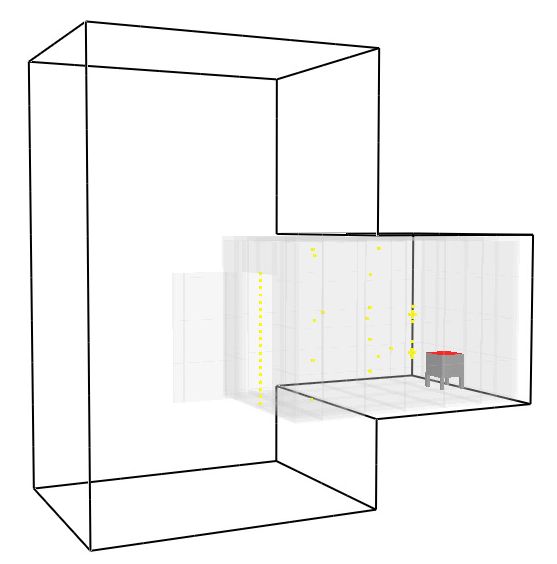
\includegraphics[trim = 5mm 5mm 5mm 5mm, clip,width=0.505\textwidth]{AOSFST_Paper/Figures/SetupDomain.png}
    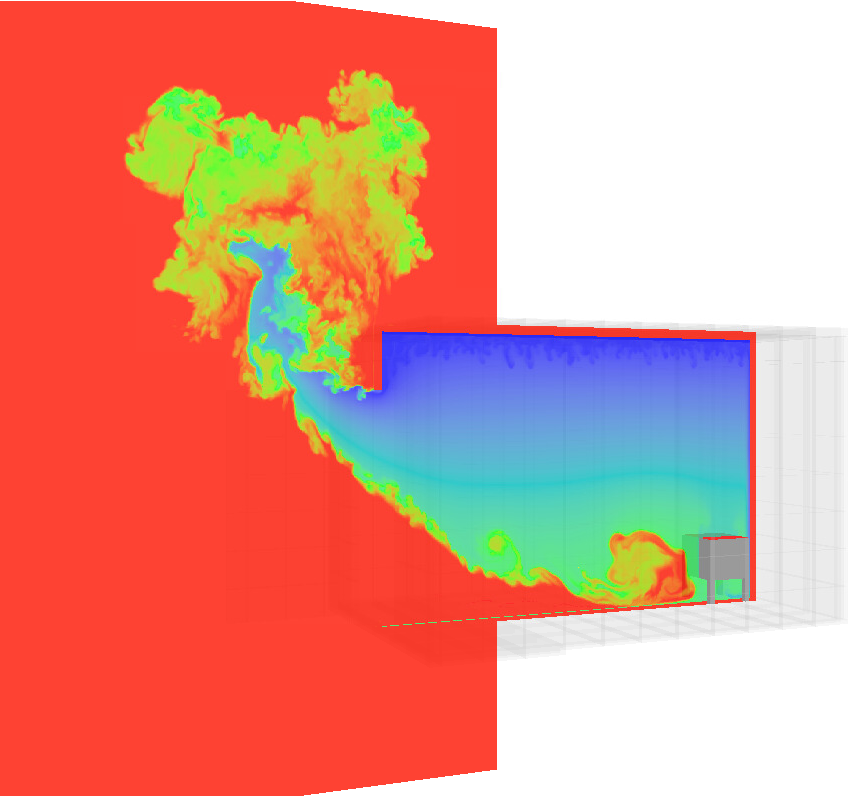
\includegraphics[trim = 22mm 5mm 17mm 5mm, clip,width=0.485\textwidth]{AOSFST_Paper/Figures/X_O2_countour_Tvar_300s_t1p5s_B.png}
    \makebox[0.50\textwidth]{(a)}
    \makebox[0.48\textwidth]{(b)} \\
    \caption{Simulation domain and geometry setup: (a) Optimized flow domain and compartment geometry, (b) Oxygen volume fraction at $t=$ sec, 0.25 cm grid resolution, FFT=300 s. Blue to red from 0.0 to 0.21. }
    \label{fig:Setupdomain}
\end{figure}

Global measures of grid sensitivity chosen are total fuel mass in the compartment $M_{C_3H_8}$ at half the simulation time t=4 s, as well as outbound fuel mass flow through the door $\dot{M}_{C_3H_8}$ and average gravity current height $H_G$. 
$H_G$ was computed as the distance from the floor where the time averaged normal velocity profile recorded in the door symmetry plane alternated sign (change form inflow to outflow). 
These give a good perspective on the mean composition evolution in the compartment and fluid mechanics resolution. Values for these quantities and differences respect to the finest  $\Delta x=0.25$ grid solution are provided in Table~\ref{tab:errgrid} for initial composition and temperature conditions gathered from the FFT=300s experiments. It is noted that all grid resolutions agree on these quantities within 5\%.

% Table of global sensitivity measures and error:
\begin{table}[h!]
\caption{Global measures of convergence for FFT=300 s, propane fuel case.}
\label{tab:errgrid}
\centering
\footnotesize
\begin{tabular}{l c c c c c c}
\hline
Grid Size & $M_{C_3H_8}$ (gr)	& $\Delta M_{C_3H_8}$ (\%) & $\dot{M}_{C_3H_8}$ (gr/s) & $\Delta \dot{M}_{C_3H_8}$ (\%) & $H_G$ (cm) & $\Delta H_G$ (\%)\\
\hline
$\Delta x=1$    cm & 62.0 & -2.2 & 6.17 & 4.53  & 47.0 & 3.1 \\
$\Delta x=0.5$  cm & 63.2 & -0.3 & 6.02 & 2.07  & 47.1 & 3.3 \\
$\Delta x=0.25$ cm & 63.5 &      & 5.89 &       & 45.6 &  \\
% Methane & 25.0~$\pm$~1.0~kW 	& 360,~390,~450\\
% 	& 37.5~$\pm$~1.0~kW 	& 225,~285      \\
% %[0.075cm]
% Propane & 16.7~$\pm$~1.0~kW		& 255,~270,~315	\\
% 	& 25.0~$\pm$~1.0~kW 	& 210,~285		 \\
\hline
\end{tabular}
\end{table}



Two ignitor locations were defined as low-ignitor (LI) and mid-ignitor (MI). The first was defined in the symmetry plane of the compartment at about 1 m from the door and 25 cm from the floor. The latter was defined also at 1 m from the door but at mid height of the compartment. Star clusters of 7 sampling devices were defined to note mixture composition and temperature at each ignitor location, and at 2 cm in every coordinate direction around it as shown in Figure~\ref{}a.

In Figures~\ref{fig:CompSetup}a,~\ref{fig:CompSetup}b local fuel and oxygen variations with time are shown at the LI, MI locations for FFT=300s and different grid resolutions. We noted on this case and others, for both LI, MI locations there was no significant difference in gas composition and temperature among the different mesh resolutions. Therefore, the analysis presented on this work is based on 1 cm grid resolution calculations.

% Figure: a) 7 point stencil of devices aroun LI ignitor location, b) LI location 300s FFT LI,MI fuel and oxygen volume fraction with time.
\begin{figure}[tb]
    \centering
    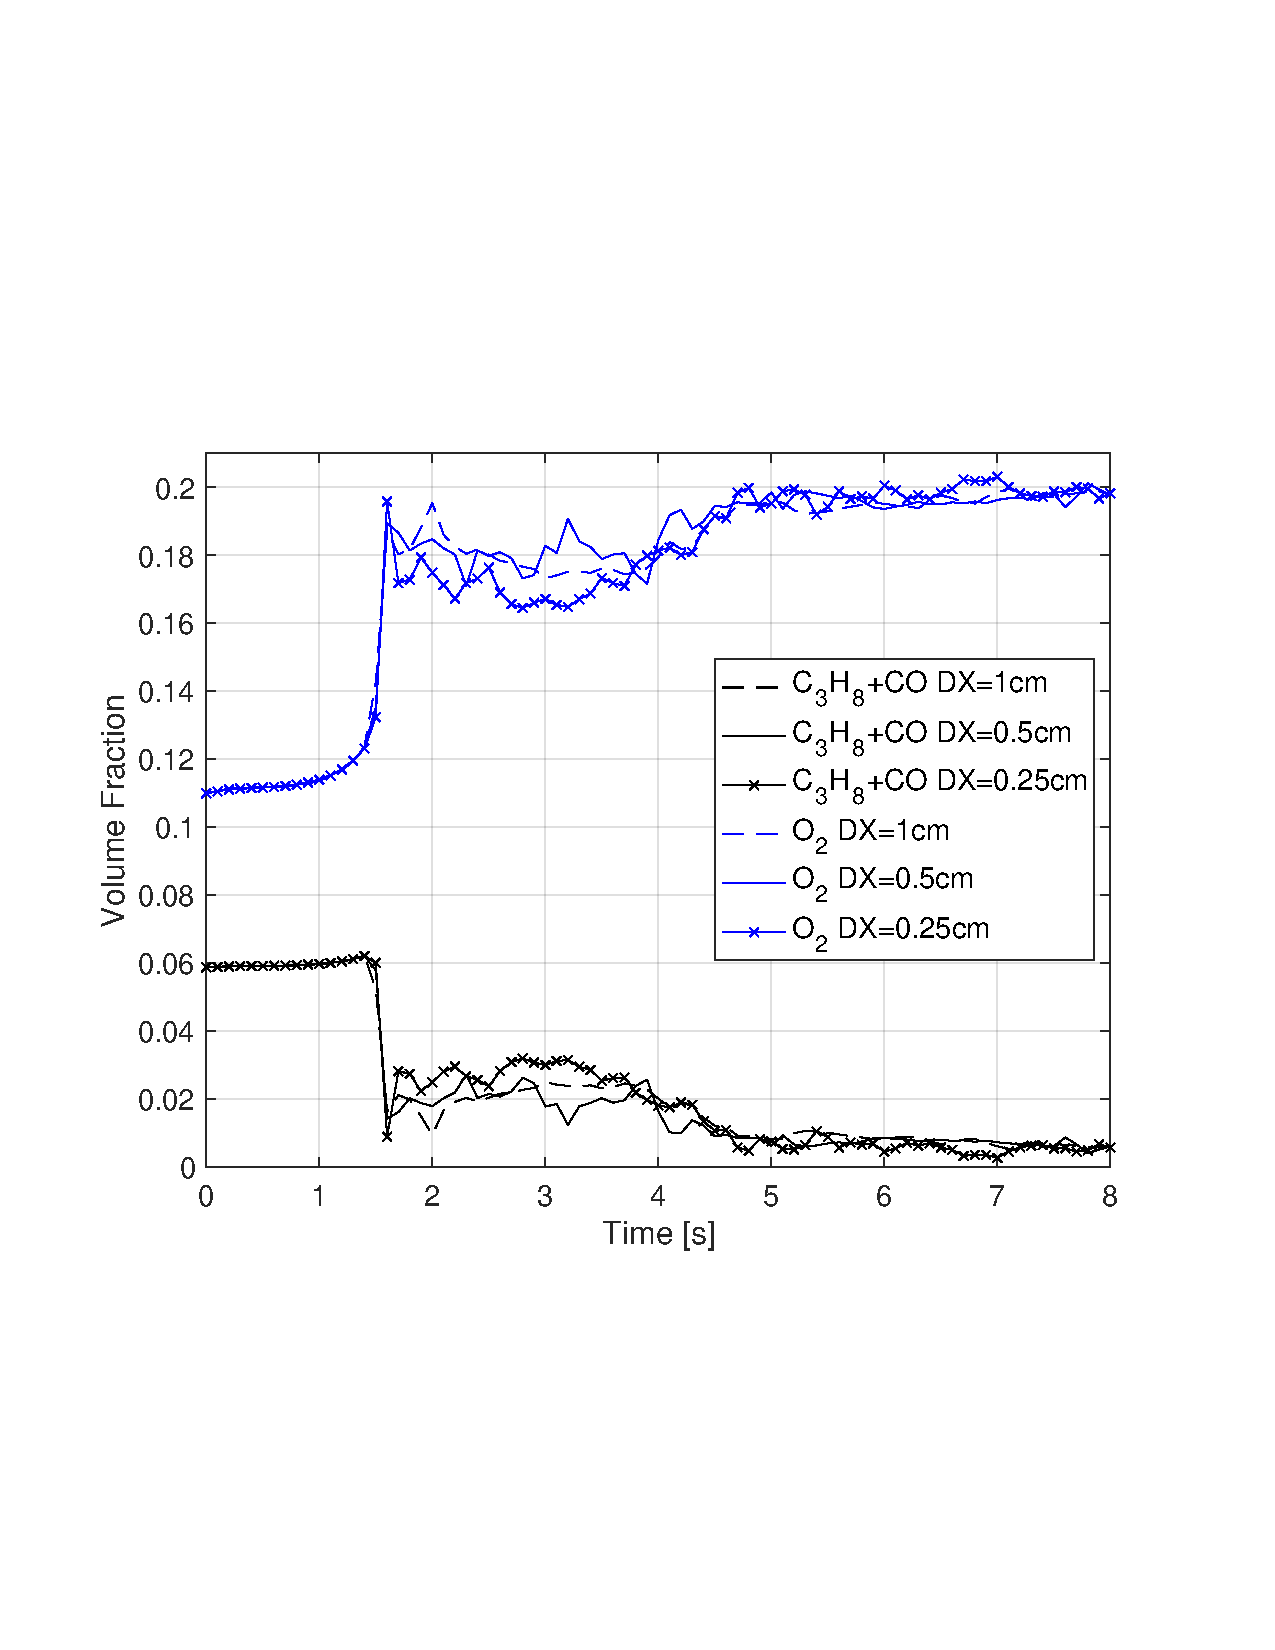
\includegraphics[trim = 14.5mm 65mm 17mm 70mm, clip,width=0.505\textwidth]{AOSFST_Paper/Figures/Low_Ignitor_Comp_Tvar_300s.pdf}
    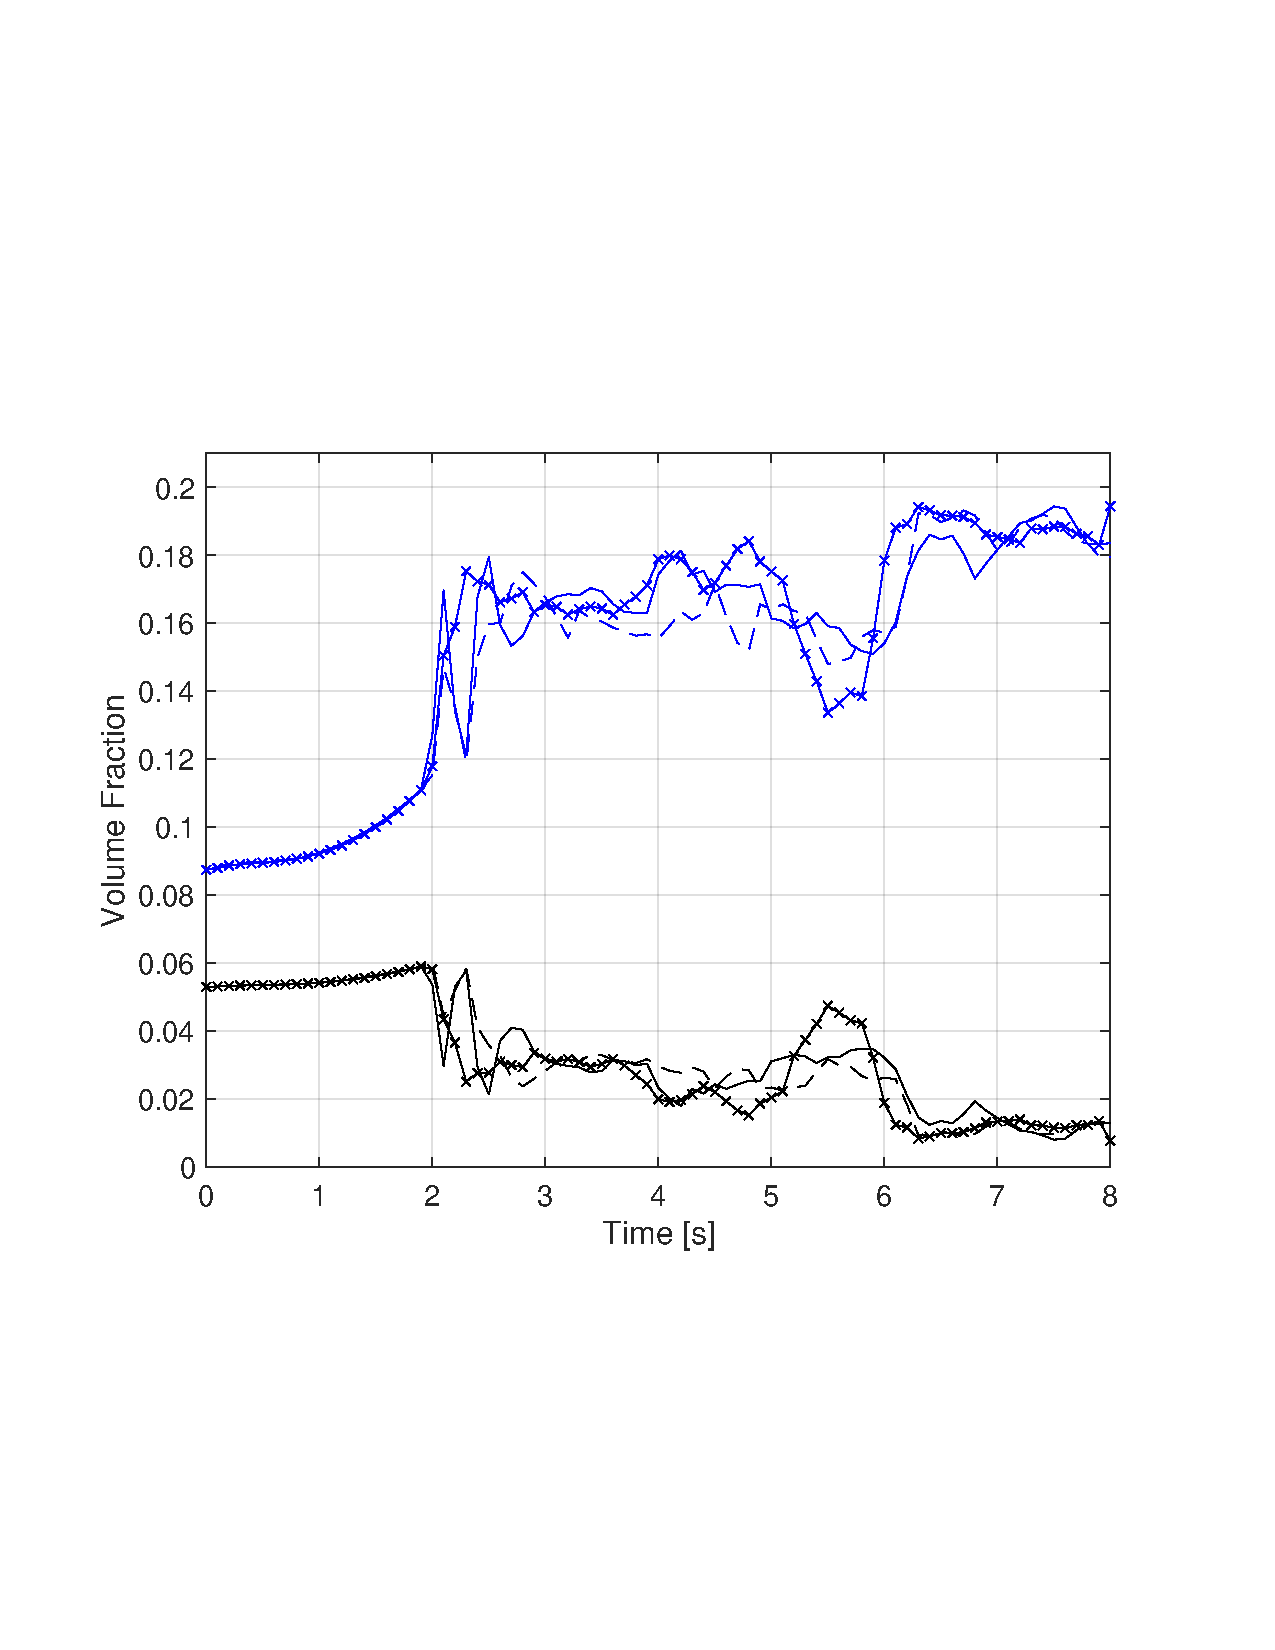
\includegraphics[trim = 22mm 65mm 17mm 70mm, clip,width=0.485\textwidth]{AOSFST_Paper/Figures/Mid_Ignitor_Comp_Tvar_300s.pdf}
    \makebox[0.50\textwidth]{(a)}
    \makebox[0.48\textwidth]{(b)} \\
    \caption{Local mixture composition as a function of time for different grid resolutions: (a) Low-ignitor (LI), (b) Mid-ignitor (MI). }
    \label{fig:CompSetup}
\end{figure}


%\textbf{-Defining conditions for flame propagation - Flammability diag/Cantera methodology}
\textbf{ Characterizing flame propagation using CANTERA tool:}

The current numerical setup aims to model a partially-premixed propane flame in an environment containing oxygen and nitrogen. Before the door was opened (i.e., before fuel flow time + 30 seconds), the enclosure can be considered a fuel-rich premixed mixture. After the door opens, gravity currents bring more oxygen into the enclosure mixture through advection and diffusion. Consequently, for combustion modeling purposes, it is considered a partially-premixed flame. Modeling such a partially-premixed flame, which can lead to a backdraft, requires capturing the flame propagation starting from the low- or mid-level ignitor. Using a detailed chemical mechanism of propane to model flame propagation can be computationally expensive. Furthermore, to accurately capture the flame thickness (~1 mm), the mesh needs to be refined further, adding to the computational cost. Therefore, to reduce computational expenses, a post-processing analysis of the enclosure conditions is performed using the CANTERA tool \cite{cantera3}. Detailed simulations using detailed chemistry and a partially-premixed flame model will be considered in future work.

In this work, the numerical simulation start at the time of door opening with the initial conditions of Fig. \ref{fig:InitCond}. We aim to determine if the mixture composition at the ignitor locations during the initial simulation period (0 to 4 seconds) can develop a flame front that propagate through the surroundings. For that, the mixture composition (temperature and species mass fractions of $\mathrm{C_3H_8, O_2, CO, CO_2, H_2O, and \ N_2}$) of low and mid ignitor points has been saved from 0 to 4 sec. Later, a detailed propane chemical mechanism \cite{Qin2000} is used in CANTERA to calculate flame related quantities (i.e., speed, Damk\"{o}hler number) for all such compositions. The post-processing analysis is presented in Section \ref{sec:CANTERAAnalysis}. 


\subsection{Results} \addvspace{10pt}
\label{sec:results}

\subsection{Effect of compartment fuel loading}
\label{sec:resfuel}


\subsection{Effect of compartment oxygen content}
\label{sec:resfuel}

\subsection{CANTERA analysis}
\label{sec:CANTERAAnalysis}

Figure \ref{fig:LI_MI_Cantera} shows the time evolution of various quantities compared between the FFT=300s and FFT=210s cases. Notably, the FFT=210s experiment did not exhibit a backdraft. In Figure \ref{fig:LI_MI_Cantera}a, at the moment of door opening (i.e., at 0 seconds), the enclosure mixture at the low and middle ignitor (LI and MI) positions is rich, which is also evident from Figs. \ref{fig:LI_MI_Cantera}c and d. Despite the high initial temperature (see Figure \ref{fig:LI_MI_Cantera}b), the rich composition does not produce a realizable flame, as confirmed by the CANTERA calculation (see Figure \ref{fig:LI_MI_Cantera}e).

Subsequently, the gravity current of low-temperature outside oxygen enters through the enclosure door, taking approximately 1.5 seconds and 2.2 seconds to reach the lower and middle ignitors, respectively. Following this, the equivalence ratio and temperature at the ignitor locations begin to drop, with the lower ignitor experiencing a more rapid decline due to the higher turbulent mixing rate.

For the FFT=300s case, the equivalence ratio at the middle ignitor mostly remains between 0.7 and 1.0 after 2.5 seconds, consistently producing a realizable flame with a flame speed of 10 to 30 cm/s (see Fig. \ref{fig:LI_MI_Cantera}e, blue solid line). During the same period, the equivalence ratio at the lower ignitor stays within the range of 0.6 to 0.75, also producing a realizable flame with a speed of approximately 10 cm/s.

In contrast, for the FFT=210s case, the equivalence ratio at the lower ignitor mostly remains below 0.5 (see Fig. \ref{fig:LI_MI_Cantera}a, red dashed line), never producing a realizable flame (see Fig. \ref{fig:LI_MI_Cantera}e, red dashed line). However, the equivalence ratio at the middle ignitor varies between 0.35 and 0.75. Therefore, at times in between 2.4 and 3.5 seconds, a realizable flame with a flame speed of 5-12 cm/s could occur. After 3.5 seconds, however, the flame speed decreases to the point where no realizable flame is produced. Note that at 3.9 seconds, the equivalence ratio at the middle ignitor is around 0.7, similar to the FFT=300s case. However, it contains less propane and more $\mathrm{CO_2}$ and $\mathrm{H_2O}$ compared to the FFT=300s case, resulting in a much lower flame speed, as shown in Fig. \ref{fig:LI_MI_Cantera}e.

Figure \ref{fig:LI_MI_Cantera}f shows the Damk\"{o}hler number (Da) at the low and middle ignitor positions for the FFT=300s and 210s cases. The Damk\"{o}hler number is the ratio of the turbulent mixing time to the chemical timescale. The turbulent mixing time is obtained from the LES turbulence model (??refer to the FDS technical guide). The chemical timescale is approximated as the ratio of flame thickness to flame speed, both of which are determined using CANTERA. When $\mathrm{Da > 1}$, the chemical timescale is shorter than the turbulent timescale, indicating that the flame can be considered in the flamelet regime, propagating with wrinkles due to turbulence. Conversely, when $\mathrm{Da << 1}$, the turbulent timescale is shorter than the chemical timescale, resulting in rapid turbulent mixing. This creates a high strain rate on the flame, potentially preventing the development of a stable flame \cite{HAMPP2019}.

For the FFT=300s case, Da remains above 10 after 3.0 seconds at the middle ignitor position, while it stays around 5 at the low ignitor position, suggesting plausible stable flame propagation. In the FFT=210s case, the Da at the low ignitor is close to zero, preventing the formation of a stable flame. Although the Da at the middle ignitor is around 5 at 2.6 seconds, it starts to decrease, and by 3.5 seconds, it becomes negligible, leading to unstable flame conditions. Please note that this is a post-processing analysis of the composition. The presence of an actual flame would introduce feedback to the flow field, which is not considered here.


\begin{figure}[!h]
\centering
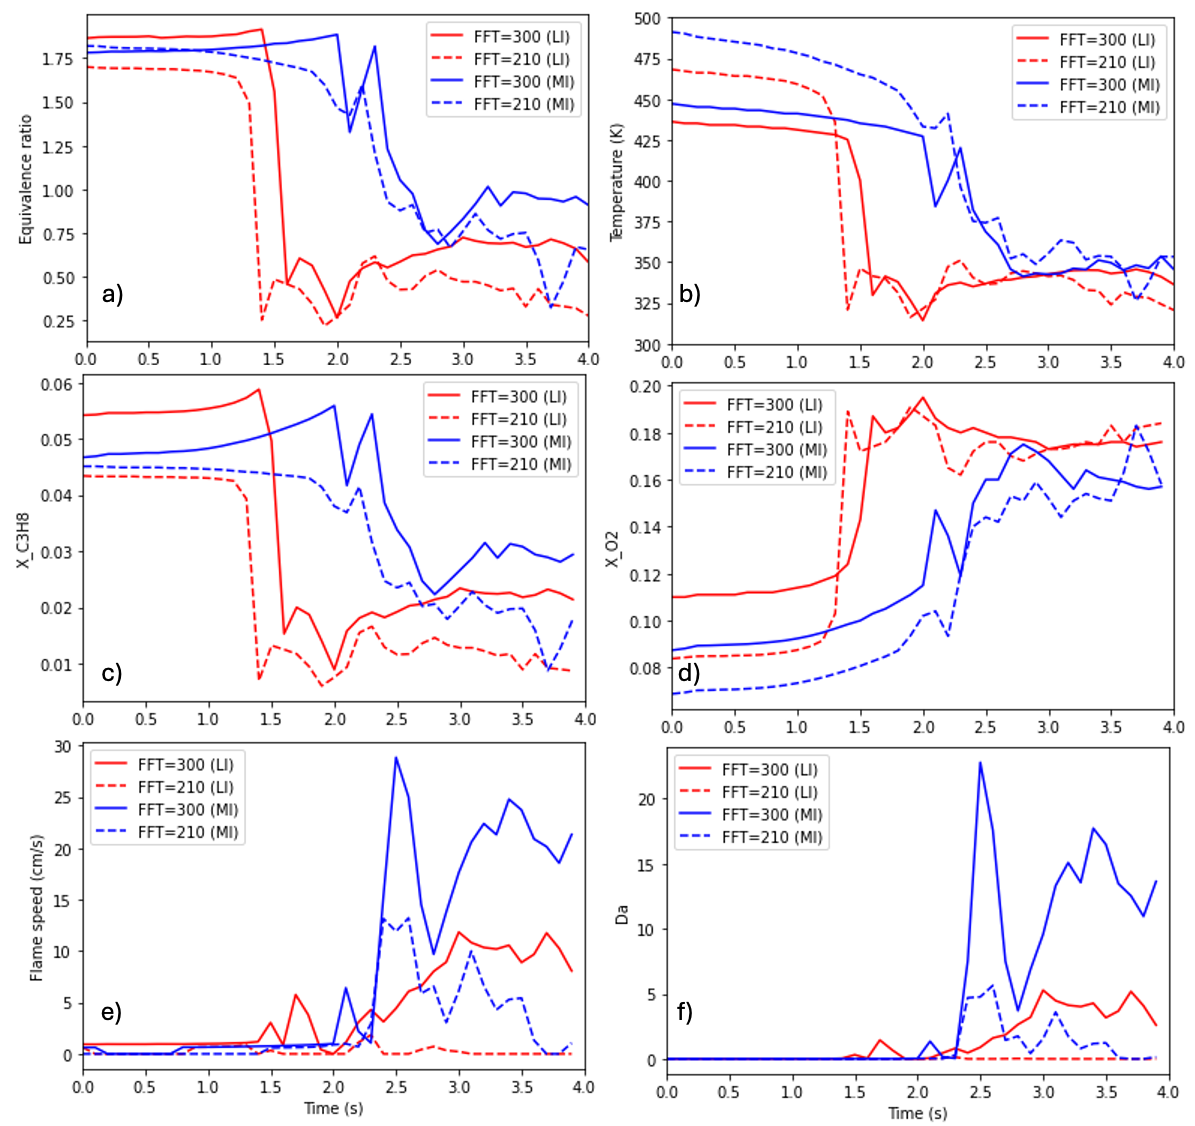
\includegraphics[scale=0.59]{AOSFST_Paper/Figures/LI_MI_Cantera.png}
\caption{Time evolution of (a) equivalence ratio, (b) temperature, (c) propane volume fraction, (d) oxygen volume fraction, (e) flame speed, and (f) Damk\"{o}hler number from 0 to 4 seconds of simulation. The solid lines represent the FFT=300s case, while the dashed lines represent the FFT=210s case. The red lines correspond to the low ignitor, and the blue lines correspond to the middle ignitor. }
\label{fig:LI_MI_Cantera}
\end{figure}

\section{Conclusions}



 

%\section*{References}
\bibliographystyle{elsarticle-num}
\bibliography{References}
\end{flushleft}
\end{document}